\section{System Design and Build Method}

Figure~\ref{fig:architecture} summarizes the six processing stages and the data passed between them.

\begin{figure*}[!t]
\centering
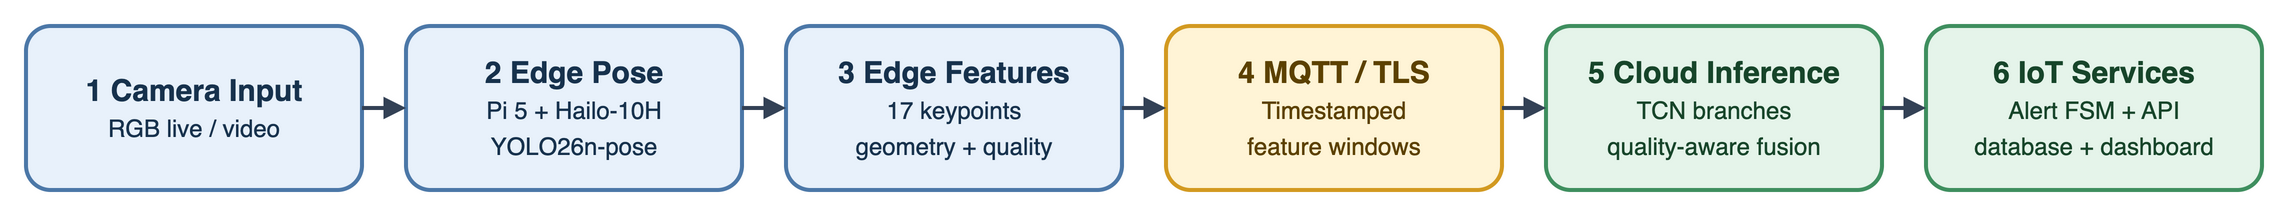
\includegraphics[width=0.98\textwidth]{figs/edge_cloud_architecture.png}
\caption{Implementation architecture and data flow. The edge transmits derived features; continuous RGB remains local.}
\label{fig:architecture}
\end{figure*}

\subsection{Datasets, Code Base, and Preparation}

UP-Fall Vision is the primary development benchmark, with falls and daily activities from 17 participants~\cite{martinez2019upfall}. GMDCSA-24 provides additional home environments, varied lighting conditions, and challenging daily-activity examples for false-positive analysis~\cite{alam2024gmdcsa}. UR Fall may be used as an additional external dataset if time permits~\cite{kwolek2014urfd}. Team-recorded non-fall clips will support the live demonstration.

Participant IDs, label mappings, and train/validation/test splits will be defined before model development and versioned for reproducibility. Each video is converted once into a cached sequence of 17 normalized keypoints, per-joint confidence, bounding-box geometry, centroid/area change, and timestamps. Fall intervals follow written transition/on-floor boundary rules.

Implementation will reuse published YOLO26 weights~\cite{jocher2026yolo26}, Hailo's pose application~\cite{hailo_yolo26_pose}, and the TCNTE repository~\cite{yu2025tcnte}. Team-developed modules will include dataset adapters, quality features, dual-branch fusion, alert logic, messaging, dashboard, and tests, keeping reused and original work traceable.

\subsection{YOLO26 Edge Pipeline}

The initial edge implementation uses Hailo's YOLO26n-pose application on the Raspberry Pi AI HAT+~2~\cite{hailo_yolo26_pose}. Its HEF and lightweight ONNX post-processing pipeline accepts live camera input. The edge callback selects the monitored person and emits normalized keypoints, bounding box, motion, pose-confidence summaries, visible-joint ratio, continuity, and missing-frame ratio. A timestamped two-second buffer is resampled to 32 steps and published every 0.5~s; RGB frames remain local. Measured throughput and latency will guide the operating resolution.

\subsection{Cloud Processing and Alert Logic}

Docker Compose will run Mosquitto, FastAPI, PostgreSQL, the inference worker, and dashboard. MQTT messages include a pseudonymous device ID, timestamps, sequence number, skeleton, geometry, and quality; TLS and per-device credentials control access.

The proposed classifier uses Branch~A for normalized skeleton trajectories and Branch~B for geometry/motion. A learned gate weights both branches from pose confidence, visibility, continuity, and missing frames. Random joint and frame masking will be evaluated as a training-time robustness augmentation, with Fall-Mamba providing related motivation for masked temporal learning~\cite{zhang2025fallmamba}. The design builds on skeleton-based temporal modeling and privacy-aware AIoT fall detection~\cite{yu2025tcnte,mobsite2024aiot}, while evaluating whether pose-quality information improves robustness under degraded visual conditions. Hyperparameters and thresholds are selected on validation subjects and then frozen.

The probability enters \textsc{Normal} $\rightarrow$ \textsc{Suspected} $\rightarrow$ \textsc{Confirmed} $\rightarrow$ \textsc{Alerted}. Confirmation requires consecutive positive windows plus sustained low position/motion; recovery cancels suspicion, and acknowledgement/cooldown prevents duplicates. The database stores transitions, predictions, device ID, and timings; the dashboard shows health, state, alerts, confidence, and latency.
